\begin{resumo}
Esse trabalho descreve o desenvolvimento de um sistema de segurança industrial que requer detecção automática de pessoas. Duas soluções baseadas em imagens de profundidade de visão superior são apresentadas. A primeira é baseada em técnicas tradicionais de aprendizado utilizando extração de características e um classificador Support Vector Machine. A segunda utiliza métodos de aprendizado profundo para classificação. A análise de desempenho das soluções demonstrou que as técnicas profundas têm desempenho supeior às tradicionais para esta tarefa ao custo de necessitarem um conjunto de treinamento maior e oferecerem maior complexidade computacional.
\end{resumo}

\begin{chave}
Detecção de pessoas, imagens de profundidade, aprendizado profundo, SVM, aprendizado de máquina, visão computacional.
\end{chave}

\begin{abstract}
This paper describes the development of an industrial safety system that requires automatic human detection. Two solutions based on top-view depth images are presented. The first one is based on traditional learning techniques using feature extraction and a Support Vector Machine classifier. The second solution uses deep learning methods for classification. The performance analysis of both solutions revealed that the deep learning methods outperform traditional learning techniques on this task, at the cost of requiring a larger training set and increased computational complexity.
\end{abstract}

\begin{keywords}
  Human detection, depth images, deep learning, SVM, machine learning, computer vision.
\end{keywords}

\section{Introdução}
  Em qualquer ambiente industrial a segurança dos funcionários deve ser garantida. Existem áreas que o oferecem maior risco e portanto não devem ser ocupadas durante a operação regular. Um exemplo ilustrativo é de uma fábrica de eletrodomésticos que utiliza uma ponte rolante superior a zona de trabalho para transportar moldes de ferro até as máquinas de extrusão de plástico. Esses moldes podem ser pesados e portanto oferecem riscos aos empregados trabalhando sob o chão da fábrica.

  Nesse contexto é útil ter um sistema de segurança automático que detecte pessoas sob o caminho da ponte e interrompa sua movimentação caso encontre uma pessoa. Uma solução baseadoa em vídeo é ideal nesse caso, especialmente considerando que o ambiente indústrial em questão é diversificadamente ocupado por máquinas, moldes e trabalhadores. Como a ponte se movimenta a câmera deve ser colocada em sua parte inferior, tendo uma vista superior do chão da fábrica. Essas condições impedem que métodos de subtração de fundo \textit{background subtraction} sejam utilizados, sendo necessário utilizar algoritmos de detecção mais sofisticados.

  Outro desafio é que as roupas dos trabalhadores não são regulares em cor, e os mesmos não necessariamente usam capacetes ou equipamentos de segurança. Nesse caso utilizar apenas imagens de cor pode não fornecer informações suficientes para detecção. A fim de superar esse problema, \cite{rauter} usa uma câmera stereo que provê imagens de profundidade dos objetos, oferecendo maior confiabilidade nas informação de forma e maior invariância à luminosidade. Essa imagem é então usada para localizar candidatos à pessoas, seguido por uma extração de características desenvolvida manualmente e posterior classificação utilizando Support Vector Machine (SVM). Entretanto, esse método pode não oferecer uma solução ideal explicitadas as considerações sobre o ambiente, visto que assume-se um ambiente limpo e estático, contrário ao ambiente industrial descrito anteriormente.

  Recentemente o aumento do poder computacional, especialmente na forma de GPUs, a disponibilização de grandes datasets de imagens e avanços em métodos de treinamento \cite{nair2010relu}, em conjunto com estruturas densas de rede \cite{NIPS2013_5207} tornou possível um rápido desenvolvimento e uso de métodos profundos de aprendizado nos mais diversos domínios, inclusive ultrapassando resultados anteriores do estado-da-arte \cite{hintonCONVNET}. A grande vantagem desses métodos é a mudança de foco da representação de características das amostras, desenvolvida manualmente até então, para um processo automático de representação, requerendo grande quantidade de amostras para oferecer um modelo adequado. Motivado por esses avanços, um segundo método de detecção de pessoas pode ser desenvolvido utilizando imagens de profundidade e classificadores profundos.

  Esse trabalho faz uma comparação entre dois métodos de detecção de pessoas, ilustrado na Figura \ref{fig:system-diagram}. Ambos utilizam técnicas de visão computacional para detectar candidatos na imagem, descritas na Seção \ref{sec:candidates}. A primeira solução, baseada em \cite{rauter}, é apresentada na Seção \ref{sec:classical}, enquanto a segunda, utilizando classificadores profundos, é descrita na Seção \ref{sec:deep}. A avaliação quantitativa dos métodos e suas variações é mostrada na Seção \ref{sec:results}. Por fim, conclusões e sugestões de trabalhos futuros são apresentadas na Seção \ref{sec:conclusion}.

  \begin{figure*}[!t]
  \centering
  \includegraphics[width=\linewidth]{system-diagram.png}
  \caption{Diagrama do sistema de detecção de pessoas.}
  \label{fig:system-diagram}
  \end{figure*}

\section{Seleção de candidatos}
\label{sec:candidates}

    Em um método tradicional de detecção de objetos \cite{traditional-objdetect} o primeiro passo é localizar os candidatos, que são em seguida validados através do processo conjunto de extração de características e classificação. No caso de uma imagem colorida, uma possibilidade para obter candidatos seria utilizar uma janela de tamanho variável que se desloca sob a imagem.

    Entretanto, ao se utilizar imagens de profundidade com visão superior, \cite{rauter} sugere um algoritmo mais eficiente que assume que as pessoas estão entre os objetos mais altos da cena. Apesar dessa hipótese nem sempre ser garantida, ela reduz significantemente o número de candidatos se comparado com o método das janelas deslocadas, e portanto será utilizada nesse trabalho e descrita a seguir.

    Primeiramente, realiza-se uma operação de máximos locais. Divide-se a imagem em blocos de tamanho especificicado e cada bloco retorna o pixel com maior intensidade, representando o ponto mais alto naquele bloco. Em seguida, para cada máximo local uma janela quadrada representando o candidato precisa ser obtida. Seu tamanho é calculado como
    \begin{equation}
      s_w = \frac{f}{d} \cdot s_r
    \end{equation}
    onde $f$ é a distância focal da câmera, $d$ a distância entre a câmera e o objeto e $s_r$ o tamanho médio da cabeça. A janela de tamanho $s_w$ pixels é centralizada em torno do respectivo pixel de máximo local.

    O último passo é a centralização da janela sob o candidato utilizando um algoritmo iterativo de \textit{mean shift}. De forma simplificada, esse algoritmo desloca a janela para o centróide dos pixels dentro dela, de forma que pixels de maior intensidade tenderão a ficar centralizados sob o candidato.

    A saída desse passo é uma lista de janelas representando os candidatos à pessoas na imagem. Um aspecto relevante a se considerar é o parâmetro de tamanho dos blocos para efetuar a busca de máximos locais. Quando se utiliza blocos muito grandes a probabilidade de ter um objeto muito alto, como uma máquina, no mesmo bloco que uma pessoa é alta, portanto aumenta-se as chances de falha de detecção. Por outro lado, quando se utiliza um bloco muito pequeno, é garantido que todas as pessoas serão consideradas candidatas, porém ao mesmo tempo eleva-se muito o número de candidatos, o que ocasiona um problema de complexidade e de performance temporal, dado que esses candidatos precisam ainda passar por validação.

\section{Solução clássica baseada em extração de características manual}
\label{sec:classical}

    Após a detecção de candidatos uma fase de validação é necessária para descartar candidatos que não são pessoas. Uma solução clássica utilizando visão computacional \cite{rauter} utiliza características extraídas por um descritor, desenvolvido manualmente, para alimentar um classificador SVM binário, que retorna uma classe: ``pessoa'' ou ``não-pessoa''. Um descritor de blocos regulares proposto em \cite{rauter} é utilizado. Para aumentar a invariância à rotação, também propomos um descritor de anéis concêntricos (veja Figura \ref{fig:descriptors}). Ambos são descritos a seguir, seguidos por mais detalhes do processo de classificação e treinamento.

    \begin{figure}
    \centering
    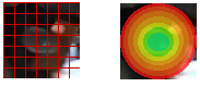
\includegraphics[width=0.9\linewidth]{tradicional/descritores}
    \caption{Descritor de grades regulares (esquerda) and anéis concêntricos (direita).}
    \label{fig:descriptors}
    \end{figure}

    \subsection{Descritor de grades regulares}
      Esse descritor divide a janela do candidato em 7x7 blocos, como ilustra a Figura \ref{fig:descriptors}. O valor médio dos pixels pertencentes à cada bloco é calculado, gerando uma matriz 7x7 de médias de intensidades de pixels. Em seguida, o valor do bloco central é subtraído da matriz. Finalmente, calcula-se o histograma da matriz resultante utilizando 32 intervalos. O vetor de histograma, com 32 dimensões, é considerado o vetor de descrição, cuja soma é 49 (número de blocos).

    \subsection{Descritor de anéis concêntricos}
       Primeiramente a janela do candidato é dividida em 18 coroas circulares (ou anéis) cujas distâncias entre os raios internos e externos é constante e cujo centro coincide com o da janela. Então calcula-se a média dos pixels pertences a cada coroa, resultando num vetor de 18 dimensões. Desse vetor subtrai-se o valor da média dos pixels da coroa mais interna (cujo raior menor é 0). Por fim, aplica-se a derivada discreta nesse vetor (subtração entre dimensões adjacentes) a fim de enunciar as diferenças entre as médias do pixels nos diferentes anéis, resultando num vetor de descrição com 17 dimensões.

    \subsection{Classificador SVM}
      Utiliza-se um classificador SVM binário com kernel \textit{Radial Basis Function (RBF)} \cite{rbfkernel} para validar os candidatos. Note que o parâmetro $\sigma$ do kernel, em conjunto com o hiper-parâmetro $C$ do SVM controlam o compromisso entre o desempenho no treinamento e a generalização do modelo em novas amostras. Valores altos de $C$ penalizam erros no conjunto de treinamento, enquanto valores menores priorizam um desempenho melhor no conjunto de teste. O parâmetro $\sigma$ tem efeito similar, porém de maneira inversa.

      A escolha dos hiper-parâmetros $C$ e $\sigma$ é feita utilizando um processo de validação cruzada com 5 conjuntos, avaliando a métrica de precisão \cite{evaluationMetrics}. Depois desse processo uma etapa de treinamento utilizando todo o conjunto de treinamento, composto de 9894 amostras negativas e 1222 positivas, é realizado. O conjunto de dados foi gerado por amostras de vídeo coletadas na fábrica durante um experimento para testar posições da câmera (fixada em uma altura de 6m). Cada amostra nesse conjunto é um recorte da janela do candidato sob a imagem de profundidade. Esses recortes foram manualmente classificados como positivos (pessoa) ou negativos (não-pessoa). O classificador SVM foi implementado em Python utilizando o toolkit Scikit-learn \cite{scikit-learn}.


\section{Solução utilizando classificadores profundos}
\label{sec:deep}

    Redes neurais artificiais podem ser utilizadas para uma classificação robusta em diferentes níveis de complexidade, variando de acordo com a estrutura e profundidade da rede. Nós utilizamos e avaliamos duas estruturas de redes profundas: perceptron multicamadas \textit{multilayer perceptron} (MLP) e redes neurais convolucionais (CNN). Em nossa solução, para ambas abordagens, o candidato é redimensionado para uma janela de 60x60 pixels and introduzido diretamente ao classificador, sem nenhum processo de extração de características inicial. Podemos considerar que o modelo desenvolve uma representação da amostra a partir das primeiras camadas da rede, sendo que a última camada é responsável pelo processo de classificação e resulta uma única saída interpretada como a probabilidade de o candidato ser uma pessoa. O diagrama dessa abordagem é o mesmo apresentado na Figura \ref{fig:system-diagram} removendo-se o bloco de extração de características e com uma saída probabilística contínua.

    \subsection{Perceptron multicamadas}
        A estrutura do MLP é composta por unidades organizadas em camadas. Cada unidade pertencente a uma camada está conectada com as unidades da camada seguinte. A saída de cada unidade é obtida calculando a soma de suas entradas ponderadas por parâmetros de conexão, seguidas da aplicação de uma função de ativação $\phi(x)$. A informação de cada unidade é propagada de forma direta pela rede desde as camadas de entrada, passando pelas camadas intermediárias até finalmente chegar na camada de saída.

        Utilizamos uma estrutura de 3600 unidades de entrada (60x60 pixels), 512 e 256 unidades nas camadas intermediárias e uma única unidade de saída, como mostra a Figura \ref{fig:diag-mlp}. As camadas intermediárias, representadas em amarelo, utilizam ativação RELU \cite{nair2010relu} de maneira a evitar o problema de gradiente enfraquecido. A únidade de saída utiliza ativação sigmóide para reproduzir uma saída de natureza probabilística.

        \begin{figure}
        \centering
        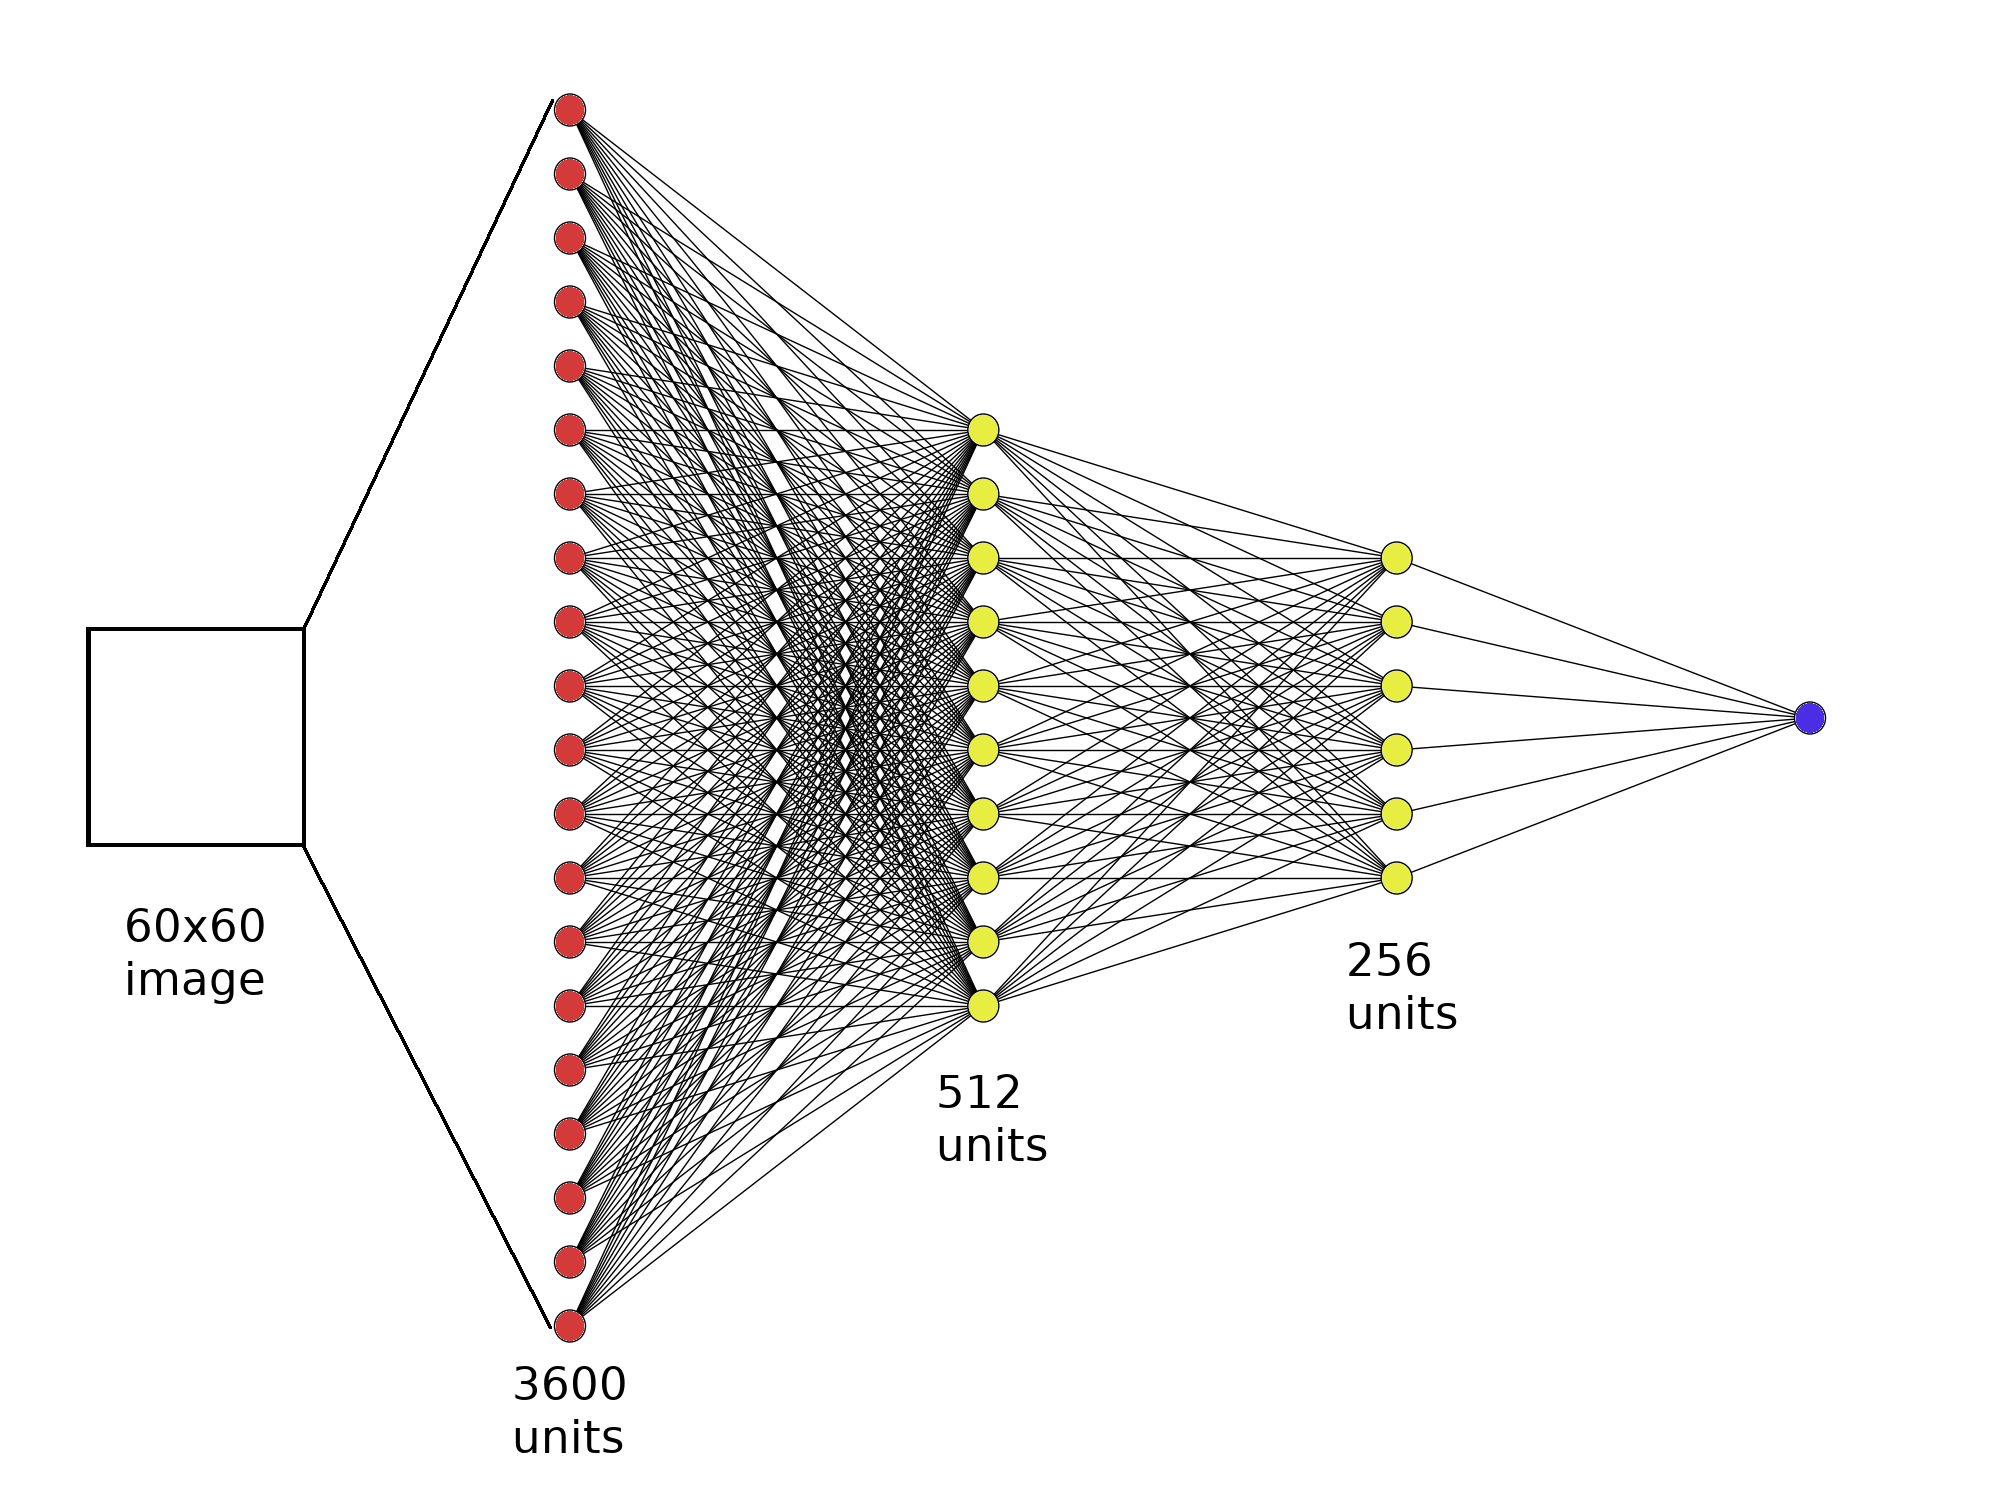
\includegraphics[width=0.8\linewidth]{diagram/diag-mlp.png}
        \caption{Estrutura MLP.}
        \label{fig:diag-mlp}
        \end{figure}

    \subsection{Rede neural convolucional}
         No caso de imagens, existe uma forte correlação entre pixels de uma redondeza, de forma que não é necessário que cada unidade de uma camada esteja conectada com todas as unidades da próxima camada, mas apenas com alguns pixels vizinhos. Esse caráter de conectividade local pode ser atingido através da convolução de uma dada camada com um banco de filtros. Nesse sentido, redes neurais convolucionais podem ser entendidas como uma derivação da MLP e, em geral, fornecem um modelo melhor para imagens através da redução do número de parâmetros e portanto aumentando ajudando na generalização.

         Nossa estrutura convolucional, ilustrada na Figura \ref{fig:diag-cnn}, é composta por uma camada convolucional 3x3 com 16 filtros, seguida por uma camada de \textit{max pooling}, e então concatenação resultando em 5776 (16x19x19) unidades seguidas por uma camada densamente ligada de 128 unidades, responsável pela classificação, e única unidade de saída que fornece uma grandeza probabilística. Novamente, as camadas intermediárias utilizam ativação RELU e a de saída utiliza sigmóide.

        \begin{figure}
        \centering
        \includegraphics[width=0.9\linewidth]{diagram/diag-cnn.png}
        \caption{Estrutura convolucional.}
        \label{fig:diag-cnn}
        \end{figure}

    \subsection{Implementação}
        O processo de treinamento consiste na minimização de uma função objetivo, nesse caso, a função de entropia cruzada binária \cite{DLbook}, também conhecida como \textit{logloss}. Seu uso é justificado pela natureza probabilística da camada de saída. O método de otimização é uma variação de \textit{Batch Stochastic Gradient Descent} (B-SGD) chamada Adam \cite{kingma2014adam}, que utiliza uma taxa de aprendizado adaptativa baseada em considerações de momento (do gradiente) para cada parâmetro de otimização.


        Como modelos de aprendizado profundo possuem muitos parâmetros e portanto requerem um conjunto de treinamento maior, extendemos o conjunto utilizado para o SVM para 16898 amostras, das quais 14966 são negativas. Um dos desafios encontrados nessa fase foi a impossibilidade de obter um modelo coerente dado a distribuição acentuadamente desbalanceada do conjunto: mais de 88\% das amostras pertencem à classe negativa, portanto o modelo classifica todas as amostras como negativas e ainda obtém uma acurácia relativamente alta. Para atacar esse problema nós artificialmente balanceamos o conjunto de treinamento replicando as amostras positivas até que a frequência dessa classe se equiparou à da classe negativa.

        As tarefas que envolvem visão computacional, extração de candidato e redimensionamento foram realizadas utilizando a biblioteca OpenCV. Ambas as estruturas de classificação profunda foram implementadas utilizando Keras \cite{keras} sob Theano \cite{theano}, que permite utilizar recursos da GPU para efetuar um treinamento rápido (aproximadamente uma época por minuto).

\section{Resultados}
\label{sec:results}

    A avaliação utiliza as curvas \textit{Receiver Operating Characteristic} (ROC) \cite{evaluationMetrics} para comparar os resultados entre soluções e parâmetros. Essas curvas são geradas através da saída probabilística dos classificadores utilizados. No caso do SVM, que sob formulação original é um classificador não-probabilístico, utilizamos uma formulação de regressão logística \cite{svmProbabilisticOutput} para obter uma saída probabilística. A grande vantagem na natureza probabilística do classificador é a possibilidade de ajustar o compromisso entre as taxas de verdadeiro positivo e falso positivo de maneira offline, após treinamento. Isso é feito através da escolha do limiar de probabilidade acima do qual a amostra é considerada positiva (pessoa).

    Para avaliar as soluções propostas nas Seções \ref{sec:classical} e \ref{sec:deep}, juntamente com suas variações, primeiramente consideramos que os candidatos já foram extraídos de uma sequência de vídeo, formando o conjunto que chamamos de teste, então avaliando apenas o descritor e o classificador. A Figura \ref{fig:result-classifiers} mostra o desempenho dos classificadores sob o conjunto de teste e a métrica \textit{Area Under Curve} (AUC) \cite{evaluationMetrics}, medida até 10\% da taxa de falso-positivo. Pode-se observar claramente que os classificadores profundos superam as técnicas de extração de características criadas de maneira manual. Apesar as estruturas MLP e CNN terem desempenho similares, um deles pode ser escolhido dependendo da região de operação que se deseja operar (maior taxa de verdadeiros-positivos ou menor taxa de falsos-positivos).

    \begin{figure*}[!t]
    \centering
    \subfloat[]{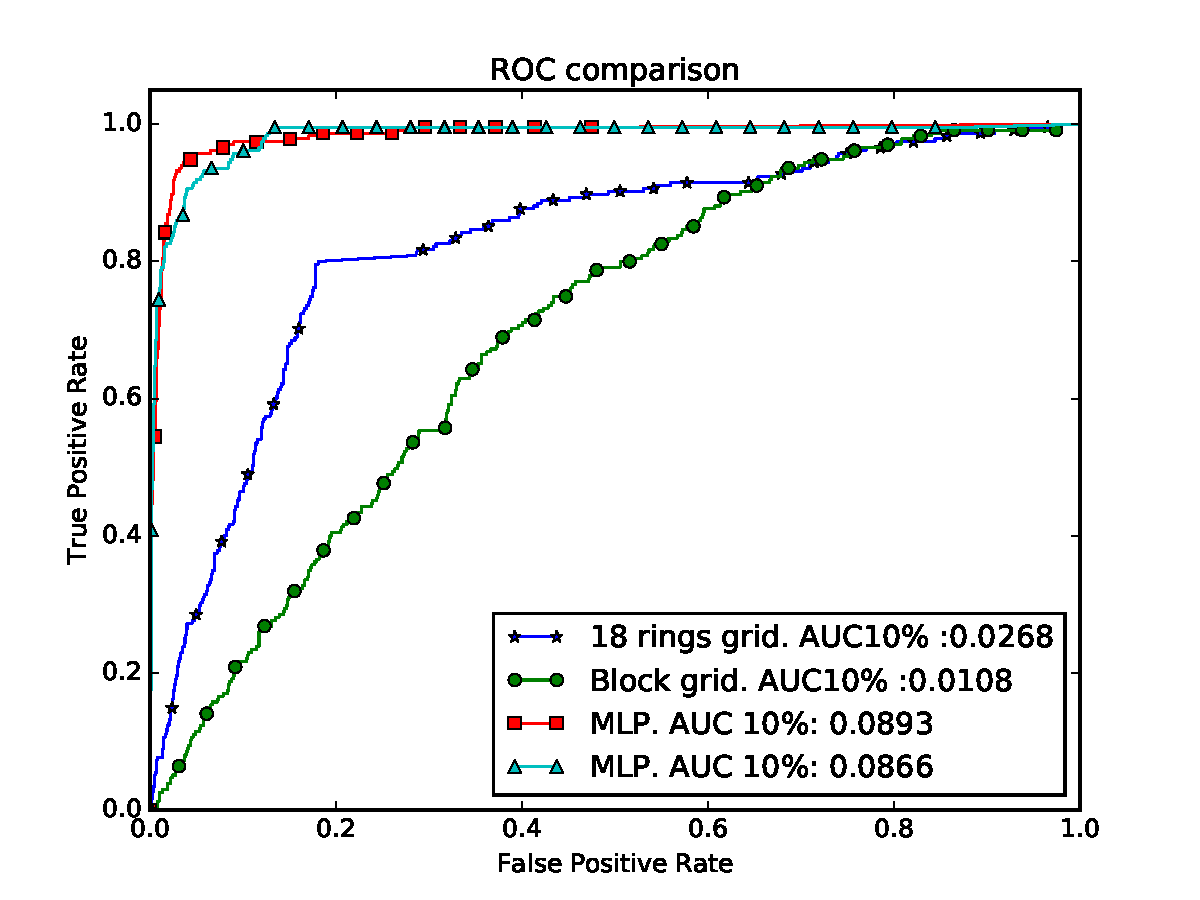
\includegraphics[width=0.45\linewidth]{results/ROC_all.pdf}}%
    \label{fig:result-classifiers-all}
    \hfil
    \subfloat[10 \% zona interesse]{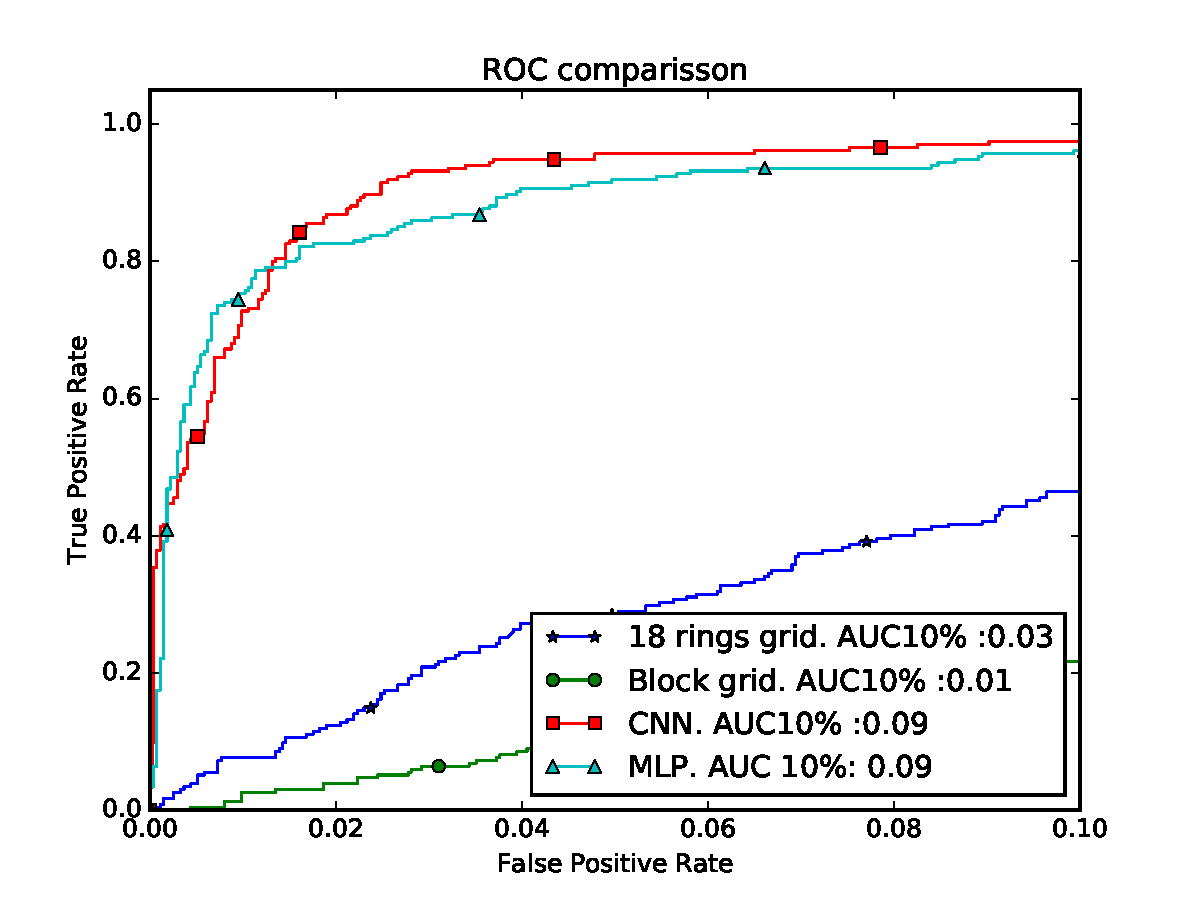
\includegraphics[width=0.45\linewidth]{results/ROC_all_zoom.pdf}}%
    \label{fig:result-classifiers-all-zoom}
    \caption{Desempenho dos classificadores.}
    \label{fig:result-classifiers}
    \end{figure*}

    Em uma segunda etapa consideramos o desempenho global do sistema, incluindo o processo de extração de candidatos. É importante notar que o desempenho observado na Figura \ref{fig:result-classifiers} é um limite superior para o desempenho global, visto que agora existirão falhas na detecção provenientes da extração de candidatos. Outra consideração é que nessa fase o conjunto de teste é composto por quadros inteiros, portanto, a probabilidade de um quadro conter pelo menos uma pessoa pode ser calculada utilizando
    \begin{equation}
    P[y=1] = 1 - \prod_i^n (1-p_i)
    \end{equation}
    onde $y$ é uma variável aleatória que assume 1 se existirem pessoas na cena ou 0 caso contrário, $n$ é o número de candidatos e $p_i$ é a saída do classificador para o candidato $i$. A Figura \ref{fig:result-system} apresenta o desempenho global do sistema utilizando essa formulação com as combinações de classificadores MLP, CNN e diferentes escalas de janelas do processo de extração de candidatos.

    Os resultados mostram que um para detector grosso (janela grande), o desempenho dos classificadores MLP e CNN são similares, porque os candidatos que são extraídos têm saídas similares. Entretanto, ao utilizar um detector fino (janela menor), muito mais candidatos são detectados, e portanto existe um número maior de amostras para explorar o desempenho desses classificadores, demonstrando que o modelo CNN tem desempenho superior ao do MLP.

    \begin{figure*}[!t]
    \centering
    \subfloat[]{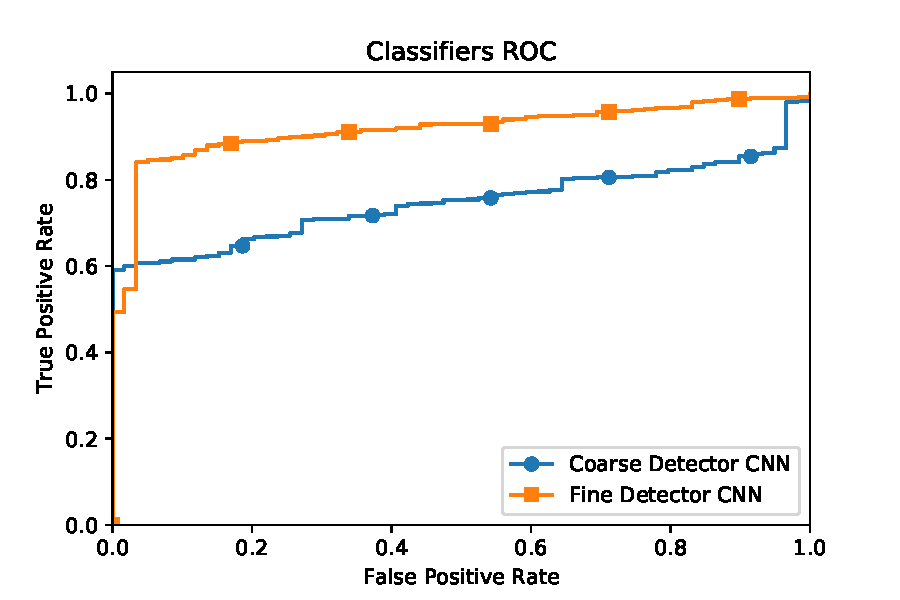
\includegraphics[width=0.45\linewidth]{results/ROC_system.pdf}}%
    \label{fig:result-system-all}
    \hfil
    \subfloat[Zona de interesse de10 \%, melhores resultados]{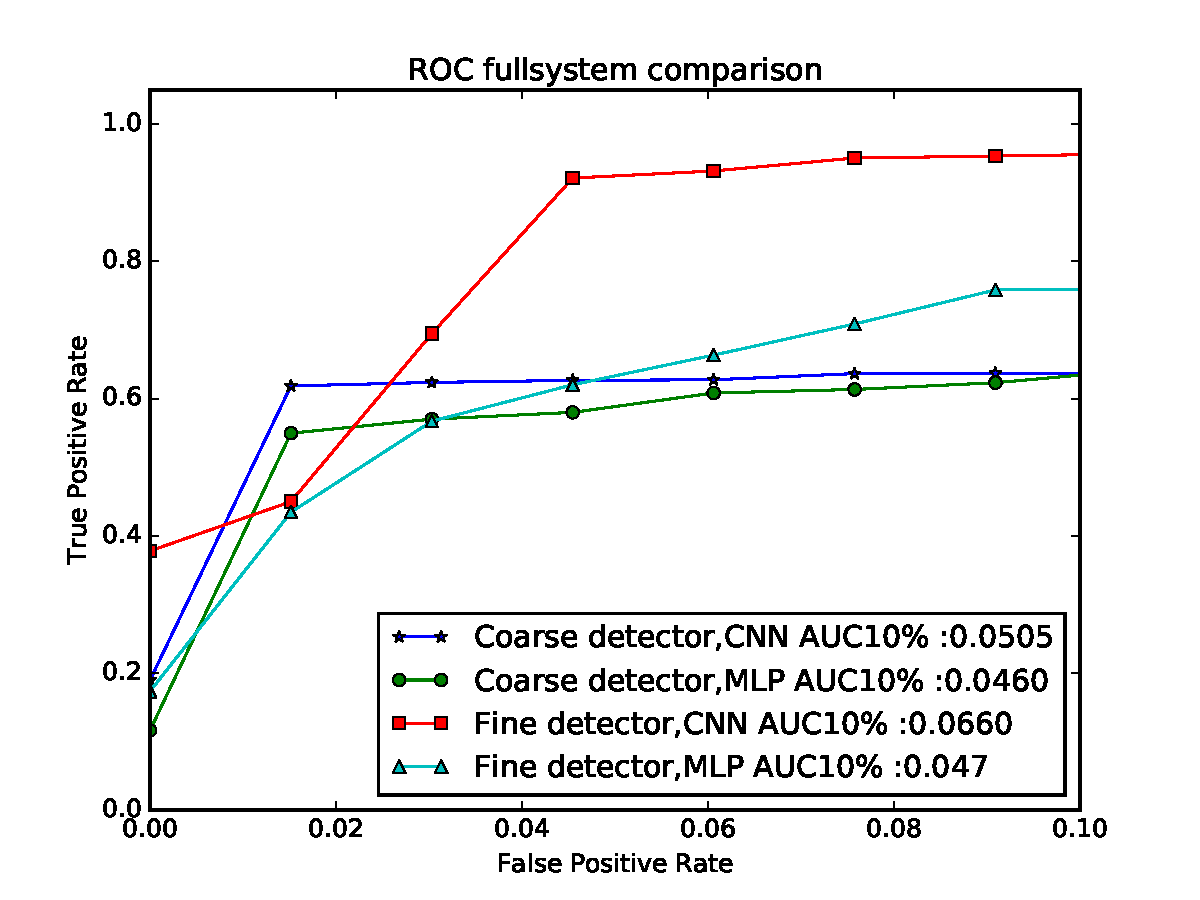
\includegraphics[width=0.45\linewidth]{results/ROC_system_zoom_best.pdf}}%
    \label{fig:result-system-all-zoom}
    \caption{Desempenho global do sistema.}
    \label{fig:result-system}
    \end{figure*}

\section{Conclusão}
\label{sec:conclusion}

    Esse trabalho investiga duas soluções para o problema de detecção de pessoas, uma baseada nas técnicas tradicionais de visão computacional e extração de características manual e outra em métodos de aprendizado profundo. Os resultados apresentados na Seção \ref{sec:results} mostram que a última solução tem desempenho superior à primeira, apesar de exigir um conjunto de treinamento maior e oferecer maior complexidade computacional, portanto requerendo mais poder de processamento. Embora as técnicas de aprendizado profundo sejam consideradas especialmente úteis para grandes datasets, nós conseguimos obter um bom resultado mesmo utilizando um conjunto de treinamento moderado e desbalanceado.

    Uma possível direção de trabalho futuro é a investigação de um modelo convolucional mais genérico. Ao invés de receber apenas a janela do candidato, essa estrutura teria acesso à imagem de profundidade completa como entrada e a saída seria a probabilidade de existir uma pessoa na cena. Assim como percebemos uma melhoria no processo de classificação permitindo ao modelo escolher a melhor representação para os dados, suspeitamos que permitir o acesso ao todo quadro, em contraposição à pequenas janelas possivelmente contendo humanos, terá um efeito positivo para o desempenho global do sistema.
